\documentclass[11pt,a4paper]{article}
\usepackage[T1]{fontenc}
\usepackage[utf8]{inputenc}
\usepackage[spanish,es-noshorthands]{babel}
\usepackage[margin=2.5cm]{geometry}
\usepackage{enumitem}
\usepackage{graphicx}
\graphicspath{{../figs/}}
\setlist{itemsep=2pt}

\title{Calibración con espectros de un fotoelectrón del Citiroc con la CAEN A5202}
\author{}
\date{\today}

\begin{document}
\maketitle

\noindent La tarjeta que usamos es una CAEN A5202 (dos Citiroc~1A, 64 canales),
controlada con el software Janus. Los nombres de los parámetros son los de
Janus (Sección~\ref{sec:janus}). Estudio número 3.

\section*{Programa de festejos}

\noindent {\bf Setup}
\begin{itemize}
\item {\bf Acción:} montar sin cristal, con los SiPM a oscuras y a 5~V de overvoltage (tensión por encima de la
  tensión de ruptura, breakdown voltage o BV). En Janus, poner los
  parámetros de la Sección~\ref{sec:janus}, con el umbral y el hold delay
  elegidos en el \emph{Hold delay scan}. Si en el \emph{Hold delay scan} la
  calibración pasó a SS de 50~ns, los pasos 1 y 3 se hacen a 50~ns con el
  hold delay de ese scan, y el paso 2 solo a 87,5~ns.
\item {\bf Resultado:} cada run se para solo a los 200\,000 eventos y lleva
  su propio número \texttt{N}. Al acabar, Janus escribe en
  \texttt{DataFilePath} \texttt{RunN\_list.csv} (para cada evento y canal,
  la baja y la alta ganancia y el tiempo de llegada, time of arrival o ToA),
  \texttt{RunN\_Info.txt} (la configuración del run) y el fichero de
  temperatura y tensión.
\end{itemize}

\noindent {\bf Paso 1: espectros de un fotoelectrón (single photoelectron,
SPE) a 5~V con el slow shaper (SS) de 25~ns}
\begin{itemize}
\item {\bf Acción:} un run con \texttt{HG\_ShapingTime} = 25~ns.
\item {\bf Resultado:} un fichero \texttt{RunN\_list.csv}.
\item {\bf Análisis:} el de la Sección~\ref{sec:analisis}: para cada canal,
  la ganancia (cuentas de ADC por fotoelectrón, pe). Es la calibración
  principal.
\end{itemize}

\noindent {\bf Paso 2: SPE a 5~V con SS de 50 y 87,5~ns}
\begin{itemize}
\item {\bf Acción:} un run con \texttt{HG\_ShapingTime} = 50~ns y otro con
  87,5~ns, cada uno con su hold delay (Sección~\ref{sec:janus}).
\item {\bf Resultado:} dos ficheros \texttt{RunN\_list.csv}.
\item {\bf Análisis:} la ganancia de cada canal con cada shaping.
\end{itemize}

\noindent {\bf Paso 3: SPE a 4 y 3~V con SS de 25~ns}
\begin{itemize}
\item {\bf Acción:} bajar el bias a 4~V de overvoltage, repetir con Janus
  la tasa de trigger frente al umbral (staircase) para fijar de nuevo el umbral en 0,5~pe (el pe es más
  pequeño), y tomar un run. Lo mismo a 3~V.
\item {\bf Resultado:} dos ficheros \texttt{RunN\_list.csv} y dos staircases.
\item {\bf Análisis:} la ganancia de cada canal a 3, 4 y 5~V; la recta de
  la ganancia frente a la tensión corta el cero en el BV de cada canal
  (Figura~\ref{fig:tension}).
\end{itemize}

\noindent {\bf Paso 4: staircase hasta 10~pe para medir crosstalk}
\begin{itemize}
\item {\bf Acción:} a 5~V, una staircase de Janus con
  \texttt{OF\_Staircase} = 1 y el rango de \texttt{TD\_CoarseThreshold}
  ampliado hasta unos 10~pe (Sección~\ref{sec:janus}). Lo mismo a 3~V,
  hasta unos 6~pe.
\item {\bf Resultado:} \texttt{RunN\_Staircase\_0\_ch.txt} para cada canal,
  con todas las mesetas.
\item {\bf Análisis:} la altura de cada meseta y el cociente entre mesetas
  consecutivas (Figura~\ref{fig:crosstalk}).
\end{itemize}

\noindent {\bf Qué necesita tu estudiante}
\begin{itemize}
\item Todo lo que hay en \texttt{DataFilePath}.
\item Logbook, una línea por run: número de run, paso al que corresponde y
  cualquier incidencia. La configuración, la temperatura y la tensión ya
  están en los ficheros de Janus.
\end{itemize}

\section{Cómo entra la medida en el modelo}
\label{sec:razon}

\begin{itemize}
\item {\bf Ganancia.} Es la unidad de toda la cadena: la simulación
  expresa cada carga en pe, y la calibración de cada canal con SPE es la
  que usará después un sistema con muchos cristales. El modelo da una
  ganancia de $0{,}93\times10^6$ electrones por voltio de overvoltage, y
  la calibración simulada recupera la ganancia de cada canal con una
  dispersión del 2\% a 25~ns (a 3~V).
\item {\bf Shaping.} Con SS largo los pulsos oscuros (dark pulses, DP) se apilan bajo el valor guardado
  y emborronan los picos. En la simulación (a 3~V) la dispersión de las
  ganancias ajustadas entre canales sube del 2\% a 25~ns al 5\% a 50~ns y
  al 7,5\% a 87,5~ns. La energía se mide en baja ganancia con 87,5~ns, así
  que la calibración con ese mismo shaping es la más directa.
\item {\bf BV.} Fija el overvoltage de cada canal y, con su coeficiente de
  temperatura (34~mV por grado), la temperatura de los SiPM. El modelo
  toma 38,0~V a 25~$^\circ$C, con una dispersión de 0,1~V típica y 0,2~V
  como mucho dentro de cada tile (matriz de 4~$\times$~4 SiPM).
\item {\bf Crosstalk.} El modelo lo trata como una ramificación: cada celda
  que se dispara, por un fotón, por un DP o por crosstalk, puede disparar a
  su vez a sus vecinas. En consecuencia los DP grandes son mucho más frecuentes
  que si cada celda disparase como mucho a otra, y eso fija la tasa de
  triggers falsos con los umbrales de los runs de energía (los runs con cristal y fuente)
  (Figura~\ref{fig:crosstalk}). La staircase hasta 10~pe distingue los dos casos.
\item {\bf Tensión.} A 5~V la ganancia es 1,67 veces la de 3~V, pero hay más
  crosstalk (19,5\% frente a 8,8\%) y los picos se emborronan más
  (Figura~\ref{fig:tension}). Los runs a 3, 4 y 5~V dicen cuál de los dos
  efectos domina.
\end{itemize}

\begin{figure}[htbp!]
\centering
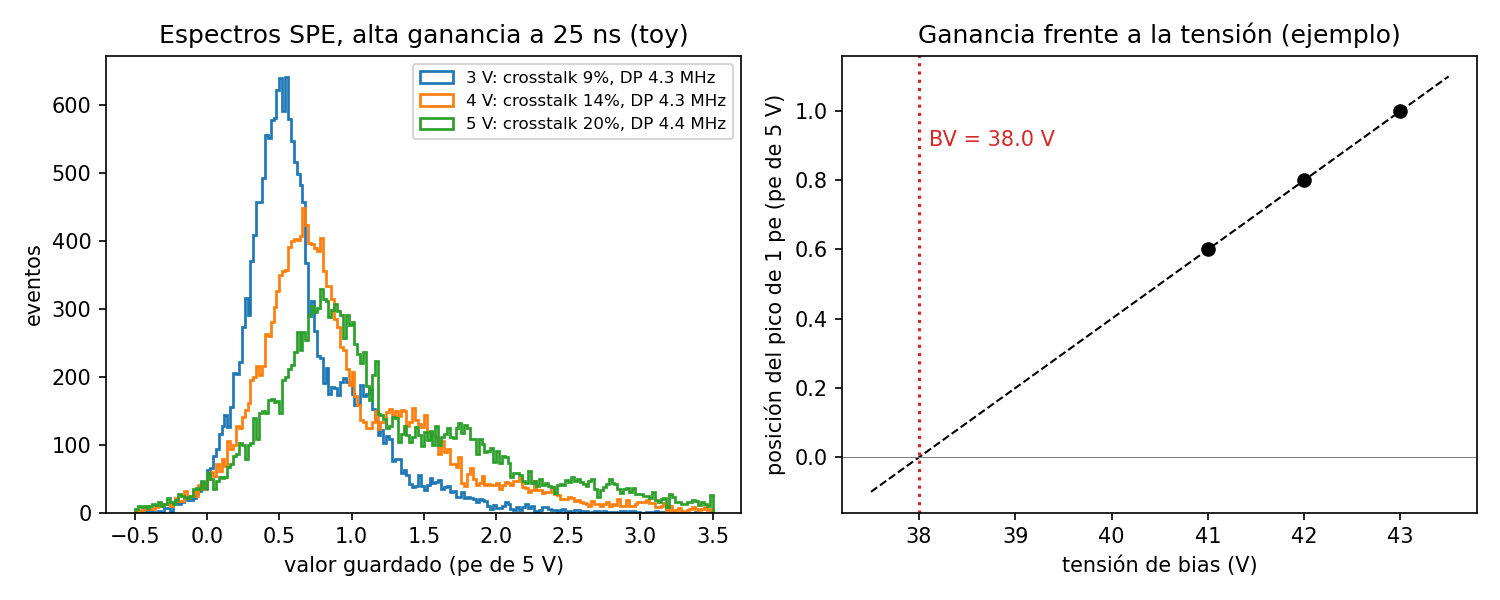
\includegraphics[width=\textwidth]{spe_tension.png}
\caption{Izquierda: espectros SPE del toy de \emph{Hold delay scan} a 3, 4 y
5~V, con SS de 25~ns y el hold en el máximo, en unidades del pe de 5~V. El
pico de 1~pe se mueve con la ganancia, y el crosstalk llena la zona de 2 y
3~pe. Derecha: la posición del pico de 1~pe frente a la tensión de bias es
una recta que corta el cero en el BV (ejemplo con BV = 38,0~V).}
\label{fig:tension}
\end{figure}

\begin{figure}[htbp!]
\centering
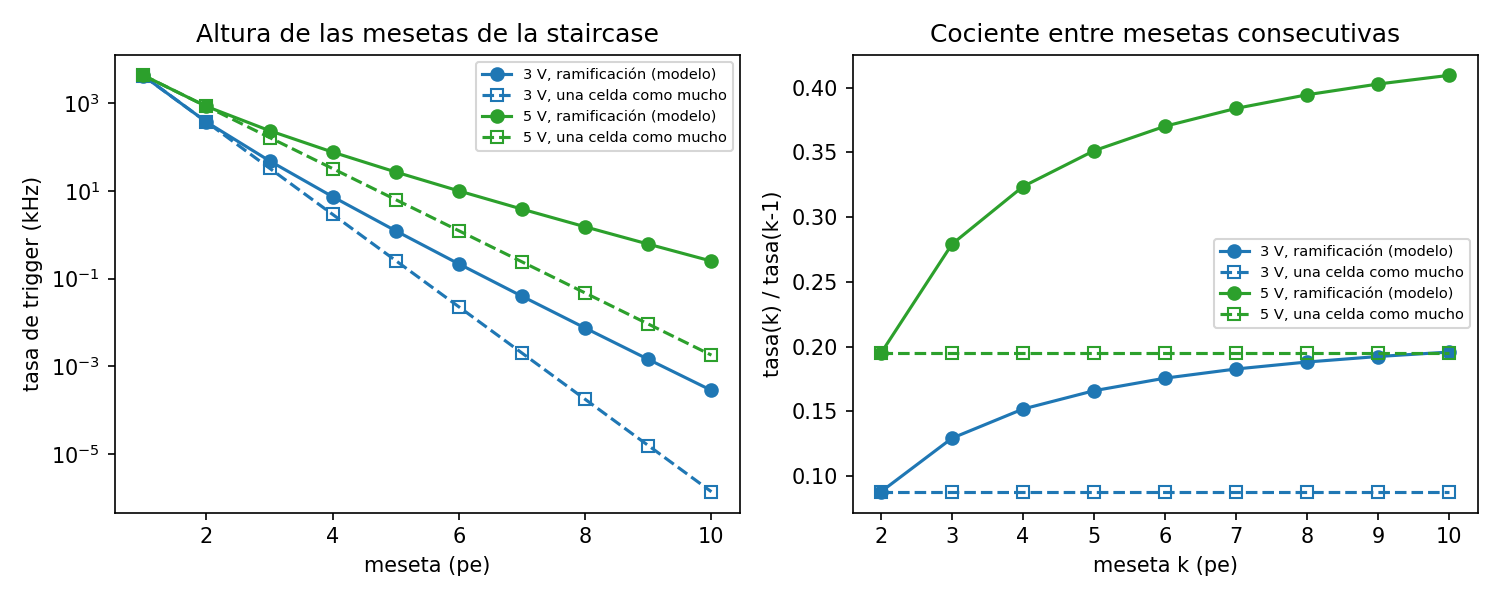
\includegraphics[width=\textwidth]{staircase_crosstalk.png}
\caption{Staircase hasta 10~pe según el modelo, a 3 y 5~V. Izquierda: altura de
las mesetas. Derecha: cociente entre mesetas consecutivas. Si cada celda
dispara como mucho a otra (cuadrados), el cociente es constante e igual a
la probabilidad de crosstalk. Con ramificación (círculos, el modelo), crece
con el número de pe: a 5~V, 0,20, 0,28, 0,32, 0,35\ldots}
\label{fig:crosstalk}
\end{figure}

\section{Parámetros de Janus (A5202)}
\label{sec:janus}

\begin{center}
\small
\begin{tabular}{p{0.3\textwidth} p{0.6\textwidth}}
\hline
parámetro & valor \\
\hline
\texttt{HV\_Vbias} & el que deje la tensión en cada SiPM 5, 4 o 3~V por
encima del BV, según el paso (unos 43, 42 o 41~V a 25~$^\circ$C si
\texttt{HV\_IndivAdj} no resta nada); \texttt{HV\_IndivAdj}: los valores que tenga cargados
la tarjeta, los mismos en los tres estudios \\
\texttt{AcquisitionMode} & SPECT\_TIMING \\
\texttt{BunchTrgSource} & T-OR \\
\texttt{TriggerLogic} & OR64 \\
\texttt{FastShaperInput} & HG-PA \\
\texttt{TD\_CoarseThreshold} & 0,5~pe, de la staircase a cada tensión \\
\texttt{PeakDetectorMode} & TRACK\&HOLD \\
\texttt{HoldDelay} & el elegido en el \emph{Hold delay scan} para 25 y
87,5~ns; para 50~ns, el de 25~ns más 27~ns, redondeado a un múltiplo de
8~ns (el máximo del pulso llega 27~ns más tarde según el modelo) \\
\texttt{HG\_ShapingTime} & 25, 50 o 87,5~ns, según el paso \\
\texttt{LG\_ShapingTime} & 87,5~ns \\
\texttt{HG\_Gain} & el mismo que en el \emph{Hold delay scan} (50 por defecto) \\
\texttt{GainSelect} & BOTH \\
\texttt{StopRunMode}, \texttt{PresetCounts} & PRESET\_COUNTS, 200000 \\
\texttt{OF\_ListCSV}, \texttt{OF\_RunInfo}, \texttt{OF\_ServiceInfo} & 1 \\
\texttt{OF\_Staircase} & 1 en los runs de staircase \\
\texttt{RunNumber\_AutoIncr} & 1 \\
\hline
\end{tabular}
\end{center}

\noindent El rango de la staircase se fija en Janus con su mínimo, su
máximo y su paso de \texttt{TD\_CoarseThreshold} y el tiempo por paso. La
distancia entre los escalones de 1 y 2~pe de la staircase a la misma tensión
(a 5~V, la del \emph{Hold delay scan}; a 3~V, la del paso 3) da el número de
unidades de DAC por pe. El máximo se pone en unos 10~pe (6~pe a 3~V), es
decir, unos 9 (5) de esos pasos por encima del escalón de 1~pe. A 5~V la meseta de 10~pe está a unos 250~Hz, así
que 500~ms por paso dan más de 100 cuentas.

\section{Análisis}
\label{sec:analisis}

\begin{itemize}
\item {\bf Espectros.} Para cada canal, el espectro de alta ganancia con
  los eventos en que fue el primero en disparar, según los ToA, como en el
  \emph{Hold delay scan}. Con 200\,000 eventos y el OR de 64 canales, unos
  3000 eventos por canal.
\item {\bf Ganancia.} Se buscan los picos de 1, 2 y 3~pe; la recta que pasa
  por sus posiciones da la ganancia (pendiente, en cuentas de ADC por pe) y
  el cero de la alta ganancia (ordenada en el origen).
\item {\bf BV.} Para cada canal, la recta de la ganancia frente a la
  tensión del canal (\texttt{HV\_Vbias} menos lo que reste su
  \texttt{HV\_IndivAdj}) con los tres puntos de 3, 4 y 5~V; su corte con el
  cero es el BV.
\item {\bf Crosstalk.} Para cada canal, la tasa de cada meseta de la
  staircase del paso 4. La primera es la tasa de DP; el cociente de la segunda
  a la primera, la probabilidad de crosstalk; los siguientes cocientes,
  si el crosstalk se ramifica.
\end{itemize}

\section{Lo que se espera, según el modelo}

\begin{itemize}
\item {\bf Ganancia:} $4{,}6\times10^6$ electrones (0,75~pC) por pe a 5~V,
  $3{,}7\times10^6$ a 4~V y $2{,}8\times10^6$ a 3~V; en cuentas de ADC
  depende de \texttt{HG\_Gain}.
\item {\bf Dispersión de las ganancias ajustadas:} la de los canales más la
  del método, que crece con el shaping (2, 5 y 7,5\% a 25, 50 y 87,5~ns en
  la simulación a 3~V).
\item {\bf BV:} 38,0~V a 25~$^\circ$C, y 34~mV menos por cada grado por debajo,
  con una dispersión de 0,1 a 0,2~V entre canales de un tile.
\item {\bf Staircase hasta 10~pe:} meseta de 1~pe a 4,4~MHz a 5~V y 4,3~MHz a
  3~V; cocientes, con ramificación, 0,20, 0,28, 0,32 y 0,35 a 5~V, y 0,09,
  0,13, 0,15 y 0,17 a 3~V.
\end{itemize}

\end{document}
